NA

NA

\begin{Schunk}
\begin{Soutput}
[1] NA
\end{Soutput}
\end{Schunk}

[1] NA

NA


[1] NA
Lo visto en la Tabla \ref{corrTableX} se refuerza claramente en la Figura \ref{corrPlotX}.

\begin{figure}[h]
\centering
\begin{adjustbox}{width=7cm,height=7cm,clip,trim=1.5cm 0.5cm 0cm 1.5cm}
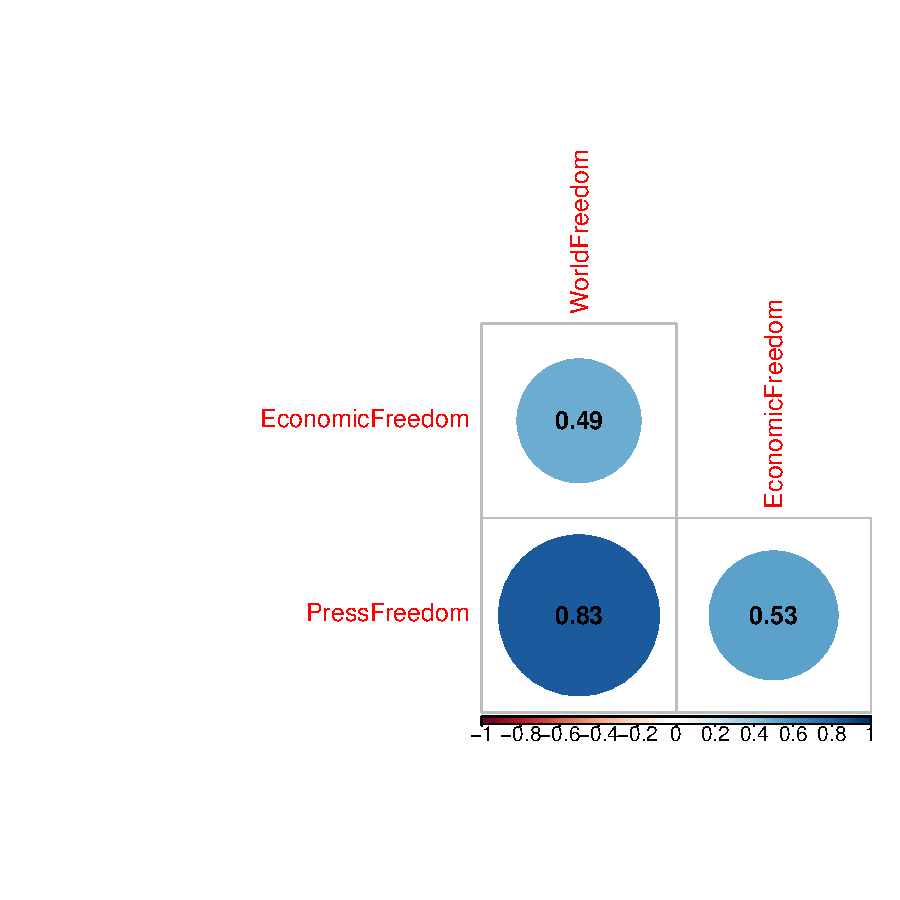
\includegraphics{paperVersion_7_bivariada-corrPlotX}
\end{adjustbox}
NA
\label{corrPlotX}
\end{figure}



\endinput
